\chapter{The \thinkhomeweather ontology}
\label{ch:thinkhomeweather_ontology}

% TODO put all names of steps according to \methontology into \emph
% TODO mention - this chapter does not cover the ontology development process as it was done; instead, it presents the completed documents that were created in that processs.
% TODO mention second paper about methontology (the one that describes all artefacts created when building the chemical ontology)

% TODO check if the things mentioned here are properly covered in the chapters referred

% TODO rename: belongsToWeatherReport -> belongsToReport

% TODO elaborate steps more?

% TODO reference paper: Building legal ontologies with METHONTOLOGY and WebODE

The previous chapters cover all topics that require discussion before being able to build a new ontology from scratch: Chapter \ref{ch:weather_data} discusses all details about weather data that is necessary and reasonable for the \thinkhomeweather ontology, what data will be used and where to obtain it. Chapter \ref{ch:existing_work} gives an overview about existing ontologies in the domain of weather data. As none of the existing ontologies being discussed fits the needs of an ontology for \thinkhome, a new ontology is to be designed. Chapter \ref{ch:development_approaches} analyzes some of the most popular approaches for building ontologies from scratch. Among those, \methontology \cite{Methontology} is identified to be the best suitable approach.

Based on these insights, this chapter describes the process of designing the \thinkhomeweather ontology in detail. The development process follows the steps proposed by \methontology as described in chapter \ref{sec:methontology}.

\section{Conventions}
\label{sec:ontology_conventions}
% TODO? \addcontentsline{toc}{section}{Conventions}

\begin{figure}
  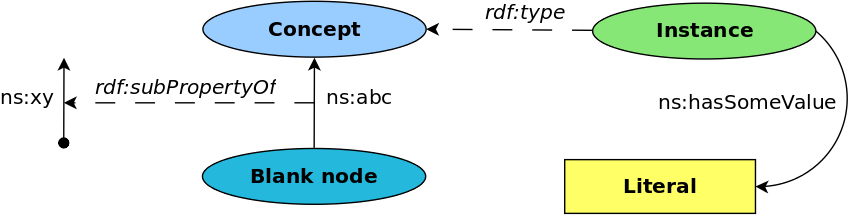
\includegraphics[width=\textwidth]{figures/diagrams/template.png}
  \caption{Example diagram}
  \label{fig:diagram_example}
\end{figure}

\definecolor{convention_color1}{HTML}{99CCFF}
\definecolor{convention_color2}{HTML}{87E776}
\definecolor{convention_color3}{HTML}{23B8DC}
\definecolor{convention_color4}{HTML}{FFFF66}
\definecolor{convention_color_bg4}{HTML}{AAAAAA}

All diagrams in this chapter showing parts of an ontology adhere to the following conventions, as seen in the example diagram shown in figure \ref{fig:diagram_example}:
\begin{itemize}
  \item \emph{Concepts} are drawn as ellipses filled with the color \texttt{\textcolor{convention_color1}{\#99CCFF}}.
  \item \emph{Instances} are drawn as ellipses filled with the color \texttt{\textcolor{convention_color2}{\#87E776}}.
  \item \emph{Blank nodes} are drawn as ellipses filled with the color \texttt{\textcolor{convention_color3}{\#23B8DC}}.
  \item \emph{Literals} are drawn as rectangles filled with the color \texttt{\colorbox{convention_color_bg4}{\textcolor{convention_color4}{\#FFFF66}}}.
  % TODO remove citations?
  \item \emph{Properties in the RDF\cite{RDF} and RDFS\cite{RDFS} namespace} are drawn as dashed lines. Their caption is written in \emph{italics}.
  \item \emph{Properties in other namespaces} are drawn as solid lines. Their caption is \emph{not} written in \emph{italics}.
\end{itemize}

% TODO cite chapter 6 of OWL 101?
% TODO naming conventions in the document
The naming conventions for identifiers within the ontology are as follows:
\begin{itemize}
  \item Two concepts, instances and/or properties may not have the same name as this is required by \emph{OWL}\cite{OWL} and avoids confusion.
  \item Two identifiers may not use names that only differ in their capitalization. Using both \emph{WeatherState} and \emph{weatherstate} in the name namespace is possible in \emph{OWL}, but leads to confusion.
  \item Identifiers may only consist of upper and lower case ASCII letters (\emph{A} to \emph{Z} and \emph{a} to \emph{z} and numerical digits from \emph{0} to \emph{9}, i.e. all identifiers must match the regular expression \texttt{\^[A-za-z0-9]+\$}.
  \item Names that are built from more than one word are written in \emph{camel case}\cite{CamelCase}, e.g. the concept representing a weather state is named \emph{WeatherState} and the property that expresses an instance of \emph{WeatherState} belongs to an instance of another concept will be named \emph{hasWeatherState}.
  \item \emph{Concepts} have an identifier that is in singular case and starts with an upper case letter. Typically a concept's identifier is a noun, e.g. \emph{WeatherState} or \emph{WeatherReport}.
  \item \emph{Properties} have an identifier that starts with a lower case letter and starts with the prefix \emph{has} or \emph{belongsTo}, followed by the name of the name of the concept which is the property's \emph{range}. The inverse property of a property having an identifier starting with \emph{has} has an identifier starting with \emph{belongsTo}, followed by the inverse property's \emph{range}, and vice versa. As an alternative to the prefix \emph{belongsTo}, the prefix \emph{is} in conjunction with the suffix \emph{Of} and the inverse property's \emph{domain} may be used.
  
  E.g. the name of a property with the domain \emph{WeatherReport} and the range \emph{WeatherState} has the name \emph{hasWeatherState}. If \emph{hasWeatherState} has an inverse property, it will have the name \emph{belongsToWeatherReport} or \emph{isWeatherStateOf}.
\end{itemize}


\section{Specification}
\label{sec:ontology_specification}

% TODO put document template in other chapter
\emph{Specification}, the first step proposed by \methontology, aims at creating an \emph{Ontology Requirements Specification Document} using natural language. It adheres to the approach discussed in chapter \ref{sec:methontology} and uses the document template taken from \cite{ORSD}.

\vspace{1em}

% TODO ensure there are no problematic page breaks inside this box (e.g. between the headline 'Scope:' and the first bullet point)
\begin{mdframed}[linewidth=.6pt]
\setlength{\parindent}{0pt}
\vspace{.3cm}

\MakeUppercase{\textbf{Ontology Requirements Specification Document}}

\vspace{.5cm}

\textbf{Name}: \thinkhomeweather

\vspace{.2cm}

\textbf{Purpose}: The ontology covers data about weather phenomena occurring at a certain location somewhere on Earth between the present and 24 hours in the future. Weather data will be acquired from both Internet services as well as from weather sensors mounted at the desired location. This weather data will enable the \thinkhome system to make decisions based on current and future weather conditions.

\vspace{.2cm}

\textbf{Scope}: The ontology has to cover a set of six core concepts from the domain of weather data:

\begin{itemize}
  \item \emph{weather phenomenon}: Represents a certain weather element. Relevant weather elements are \emph{temperature}, \emph{humidity}, \emph{dew point}, \emph{wind speed} and \emph{direction}, \emph{precipitation intensity} and \emph{probability}, \emph{atmospheric pressure}, \emph{cloud cover}, \emph{solar radiation}, and the \emph{sun's position}.
  \item \emph{Weather condition}: Overall state of the weather given by a simple verbal description: \emph{sun}, \emph{light clouds}, \emph{partly cloudy}, \emph{cloudy}, \emph{fog}, \emph{rain}, \emph{snow}, \emph{sleet}, \emph{thunder}.
  \item \emph{Weather state}: Summarizes all weather phenomena for a certain time. 
  \item \emph{Weather report}: Summarizes all data acquired at a certain time about the current weather or the weather some time in the future. Exactly one \emph{weather state} is linked to each \emph{weather report}.
  \item \emph{Weather report source}: Source where the data belonging to a \emph{weather report} has been obtained from (either an Internet weather service or a local weather sensor).
\end{itemize}

\vspace{.2cm}

\textbf{Implementation language}: The ontology is implemented in \emph{OWL 2.0}\cite{OWL} using \protege\footnote{\href{http://protege.stanford.edu/}{http://protege.stanford.edu/}} and the \emph{Pellet reasoner}\footnote{\href{http://clarkparsia.com/pellet/}{http://clarkparsia.com/pellet/}}.

\vspace{.2cm}

% TODO reformulate
\textbf{Intended end-users}: The ontology is part of the \thinkhome project. Hence, any user of the \thinkhome project is a user of the \thinkhomeweather ontology. \thinkhome aims at providing home automation to \emph{house occupants}; therefore, every occupant of a house is a possible end user for \thinkhomeweather. However, he/she will never have to deal with any ontology. \thinkhome is ought to make decisions on itself based on the knowledge acquired from the \thinkhomeweather ontology. Only the \emph{developers of \thinkhome} have to deal with the ontology itself.

\vspace{.2cm}

\textbf{Intended uses}: The ontology shall provide knowledge to \thinkhome about the current and future state of the weather in order to enable \thinkhome to make decisions based on that knowledge.

\vspace{.2cm}

\textbf{Ontology requirements}:

\vspace{.2cm}

\setlength{\leftskip}{.5cm}

\textbf{Non-functional requirements}:

\begin{itemize}
  \item The ontology must adhere to the naming conventions presented in section \ref{sec:ontology_conventions} regarding the identifiers that may be used for classes, properties and individuals.
  \item The ontology must be documented thoroughly in order to make it easily reusable.
  \item The ontology must re-use existing ontologies wherever possible.
\end{itemize}

\textbf{Functional requirements}: The functional requirements are covered by the competency questions that the ontology shall be able to answer (see section \ref{sec:weather_information}):

\begin{itemize}
  \item What is the current weather situation?
  \item What will the weather situation be in one hour, in two hours, …, in 24 hours?
  \item What is the current temperature, humidity, wind speed, …?
  \item What will be the temperature, humidity, wind speed, … in one hour, in two hours, …, in 24 hours?
  \item What will be the minimum temperature, humidity, … over the next 24 hours? What about maximum values?
  \item Will the weather change? Will the temperature, humidity, … rise or fall?
  \item Does it rain? Will it rain in the next hours? Will it rain today?
  \item Will there be sunshine today? 
  \item Do we need to irrigate the garden?
  \item Will there be severe weather?
  \item Will temperature drop/stay below $0^\circ C$?
  \item When can we open windows and when do we have to keep them shut?
  \item When do we need sun protection?
  \item When will it outside be colder than inside the house? When will it be warmer?
\end{itemize}

\setlength{\leftskip}{0cm}

\vspace{.2cm}

\textbf{Pre-glossary of terms}: These are all terms that can be extracted from the competency questions, in alphabetical order:

24 hours, airing, current weather, frost, future weather, humidity, humidity rise, humidity fall, irrigation, minimum, maximum, rain, room temperature, severe weather, sunshine, sun protection, temperature, temperature rise, temperature fall, weather change, wind speed.

\setlength{\leftskip}{0cm}

\end{mdframed}

\vspace{.5cm}

In the following sections, the \thinkhomeweather ontology is built in a way to meet all above requirements, if possible. Section \ref{sec:ontology_evaluation} evaluates if the resulting ontology fits the specification and which shortcomings the ontology comes with.

\section{Knowledge Acquisition}

The second step proposed by \methontology is \emph{Knowledge Acquisition}. All knowledge required to build the \thinkhomeweather ontology is presented in the chapters~\ref{ch:existing_work} and~\ref{ch:weather_data}. These chapters discuss in detail:

\begin{itemize}
  \item Which weather data are relevant for \thinkhome?
  \item Which weather data are available from sensors (section~\ref{sec:weather_sensors}) and Internet services (section~\ref{sec:internet_services})? How can this data be acquired?
  \item Which data do not have any use for \thinkhomeweather due to being too complicated or because they cannot be processed in an ontology in a useful way?
  \item What knowledge about weather in general is required to build an appropriate ontology? % TODO check if this is available in the previous chapters
\end{itemize}

Furthermore, chapter~\ref{ch:existing_work} covers existing ontologies that cover the domain of weather data. An additional source of knowledge is available through works about weather in general, e.g. the \emph{Glossary of Meteorology}\footnote{\href{http://glossary.ametsoc.org/wiki/Main\_Page}{http://glossary.ametsoc.org/wiki/Main\_Page}} by the \emph{American Meteorological Society}\footnote{\href{http://www.ametsoc.org/}{http://www.ametsoc.org/}}\cite{GlossaryOfMeteorology}.

\section{Conceptualisation}

In the third step of \methontology, the \emph{Conceptualisation} step, the domain knowledge is structured into a conceptional model that describes the problem and its solution in terms of the domain vocabulary that has been identified in the \emph{Specification} process.

The starting point of \emph{Conceptualisation} is a complete \emph{Glossary of Terms} that covers all concepts, instances, attributes and binary relations that will form the ontology.

\subsection{Glossary of Terms}
\label{sec:ontology_glossary}

When describing the scope of \thinkhomeweather, the \emph{Ontology Requirements Specification Document} in section~\ref{sec:ontology_specification} mentions five top-level concepts (i.e. concepts that do not have a superclass except \emph{Thing} in \emph{OWL}) of the ontology: \Egls{weather report}, \Egls{weather state}, \Egls{weather phenomenon}, and \Egls{weather condition}. All other concepts are sub-concepts of these five concepts.

In this section, only a list of terms is given; the complete \emph{Glossary of Terms} with short descriptions of each term can be found in the appendix~\ref{main} which starts on page~\pageref{main}.

\paragraph{Concepts:}

% TODO link to section/subsection?
Section~\ref{ch:weather_data} discusses each weather element that is used in \thinkhomeweather and categories in which its instances can be grouped into. In the ontology, all weather elements are represented by concepts that sub-concepts of \Egls{weather phenomenon}. All categories of weather elements are in turn sub-concepts of the weather elements' concepts.

A \egls{weather report} can encapsulate data either about the current weather or about the weather some time in the future which is specified by its \egls{start time}. Additionally, weather data can origin at a set of weather sensors or at an Internet weather service. To take this into account, a few sub-concepts of \egls{weather report} are introduced:

If the \egls{weather report} describes the current weather, it is a \Egls{current weather report}; if it describes the future weather, it is a \Egls{forecast weather report}. Depending on how far the \Egls{weather report}'s \egls{start time} lies into the future, it is a \Egls{short range weather report} (at most 3 hours in the future), a \Egls{medium range weather report} (more than 3 hours and less than 12 hours in the future) or a \Egls{long range weather report} (at least 12 hours in the future). % TODO additional concepts

If the source of weather data is a \Egls{sensor source}, the corresponding \Egls{weather report} is a \Egls{weather report from sensor}; otherwise (if the source of weather data is a \Egls{service source}), it is a \Egls{weather report from service}.

A \Egls{weather report} that is both a \Egls{current weather report} and a \Egls{weather report from sensor} is a \Egls{current weather report from sensor}. A \Egls{weather report} that is both a \Egls{current weather report} and a \Egls{weather report from service} is a \Egls{current weather report from service}.

% TODO additional sub-concepts of Weather states

Hence, these are the concepts that can be found in \thinkhomeweather are:
\begin{itemize}
  \item \Egls{weather condition}
  \item \Egls{weather phenomenon}:
    \begin{itemize}
      \item \Egls{atmospheric pressure}: \Egls{very low pressure}, \Egls{low pressure}, \Egls{average pressure}, \Egls{high pressure}, \Egls{very high pressure}
      \item \Egls{cloud cover}: \Egls{clear sky}, \Egls{partly cloudy}, \Egls{mostly cloudy}, \Egls{overcast}, \Egls{unknown cloud cover}.
      \item \Egls{dew point}.
      \item \Egls{humidity}: \Egls{very dry}, \Egls{dry}, \Egls{normal humidity}, \Egls{moist}, \Egls{very moist}.
      \item \Egls{precipitation}: \Egls{no rain}, \Egls{light rain}, \Egls{medium rain}, \Egls{heavy rain}, \Egls{extremely heavy rain}, \Egls{tropical storm rain}.
      \item \Egls{solar radiation}: \Egls{no radiation}, \Egls{low radiation}, \Egls{medium radiation}, \Egls{high radiation}, \Egls{very high radiation}.
      \item \Egls{sun position}: \Egls{day}, \Egls{solar twilight}, \Egls{twilight}, \Egls{civil twilight}, \Egls{nautical twilight}, \Egls{astronomical twilight}, \Egls{night}, \Egls{sun from north}, \Egls{sun from east}, \Egls{sun from south}, \Egls{sun from west}.
      \item \Egls{temperature}: \Egls{frost}, \Egls{cold}, \Egls{below room temperature}, \Egls{room temperature}, \Egls{above room temperature}, \Egls{heat}.
      \item \Egls{wind}: \Egls{directional wind}, \Egls{north wind}, \Egls{east wind}, \Egls{south wind}, \Egls{west wind}, \Egls{calm}, \Egls{light wind}, \Egls{strong wind}, \Egls{storm}, \Egls{hurricane}.
    \end{itemize}
  \item \Egls{weather report}: \Egls{weather report from sensor}, \Egls{weather report from service}, \Egls{current weather report}, \Egls{current weather report from sensor}, \Egls{current weather report from service}, \Egls{forecast weather report}, \Egls{short range weather report}, \Egls{medium range weather report}, \Egls{long range weather report} % TODO additional concepts
  \item \Egls{weather source}: \Egls{sensor source}, \Egls{service source}.
  \item \Egls{weather state} % TODO additional concepts
\end{itemize}

\paragraph{Relations:}

Instances of the concepts are associated to each other with binary relations, which are:

\begin{itemize}
  \item \egls{has source} and \egls{is source of} which connect instances of \Egls{weather report} and \Egls{weather source}.
  \item \egls{has weather state} and \egls{belongs to weather report} which connect instances of \Egls{weather report} and \Egls{weather state}.
  \item \egls{has condition} which connects instances of \Egls{weather state} and \Egls{weather condition}.
  \item \egls{has weather phenomenon} and \egls{belongs to state} which connect instances of \Egls{weather state} and \Egls{weather phenomenon}.
  \item \egls{has previous weather state} and \egls{has next weather state} which connect two instances of \Egls{weather state}.
\end{itemize}

The following relations link instances of concepts from other ontologies than \thinkhomeweather to instances of concepts inside the ontology: \egls{has start time}, \egls{has end time}, \egls{has observation time}, and \egls{location}.

The only data property in \thinkhomeweather is \egls{has priority} which specifies an integer value indicating which \Egls{weather report} for a certain period of time is to be preferred over another \Egls{weather report} for the same period of time.

\paragraph{Individuals:}

The only predefined individuals are instances of the concept \Egls{weather condition}; they represent the overall state of the weather for a certain \Egls{weather state}. These individuals are: \emph{cloud}, \emph{fog}, \emph{light clouds}, \emph{partly cloudy}, \emph{rain}, \emph{sleet}, \emph{snow}, \emph{sun}, and \emph{thunder}.

\subsection{Concept-classification trees}
\label{sec:concept_classification_trees}

As stated in section~\ref{sec:ontology_glossary}, there are fix top-level concepts; all other concepts are sub-concepts to these top-level concepts. As a consequence, each of these concepts becomes root of a tree of concepts. These \emph{Concept-classification trees} are presented in this section.

A \Egls{weather condition} does not have any sub-concepts. Hence, its classification tree which is shown in figure~\ref{fig:tree_weather_condition} looks rather simple.

\begin{figure}
  \centering
  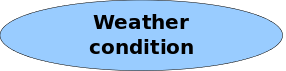
\includegraphics[width=.3\textwidth]{figures/diagrams/weather-condition.png}
  \caption{Concept-classification tree for \Egls{weather condition}}
  \label{fig:tree_weather_condition}
\end{figure}

A \Egls{weather phenomenon} represents a certain weather element. Every specific weather element is a sub-concept of \Egls{weather phenomenon}; the evolving tree is shown in~\ref{fig:tree_weather_phenomenon}. For sake of clarity, this tree is broken up to several diagrams; all sub-concepts of sub-concepts of \Egls{weather phenomenon} are not shown in~\ref{fig:tree_weather_phenomenon}. There is a separate diagram for each sub-concept of \Egls{weather phenomenon}: \Egls{atmospheric pressure} (figure~\ref{fig:tree_atmospheric_pressure}), \Egls{cloud cover} (figure~\ref{fig:tree_cloud_cover}), \Egls{humidity} (figure~\ref{fig:tree_humidity}), \Egls{precipitation} (figure~\ref{fig:tree_precipitation}), \Egls{solar radiation} (figure~\ref{fig:tree_solar_radiation}), \Egls{sun position} (figure~\ref{fig:tree_sun_position}), \Egls{temperature} (figure~\ref{fig:tree_temperature}), and \Egls{wind} (figure~\ref{fig:tree_wind}). The diagram for \Egls{dew point} is not shown as that concept does not have any sub-concepts; hence its concept-classification tree consists of a single node.

\begin{figure}
  \centering
  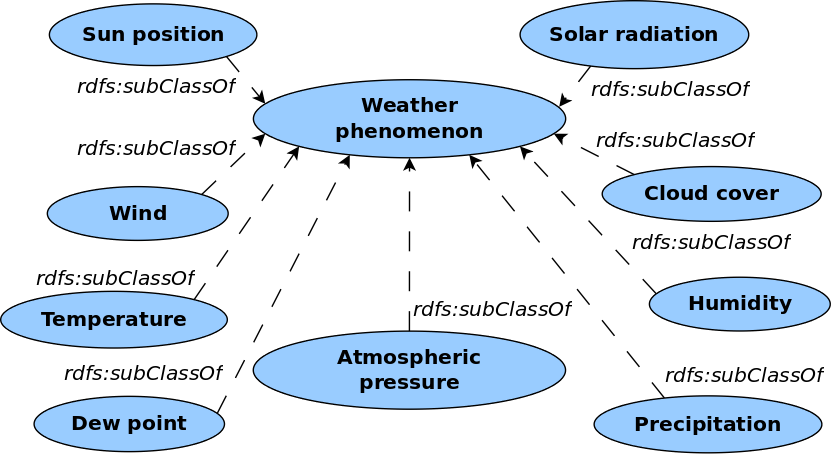
\includegraphics[width=.8\textwidth]{figures/diagrams/weather-phenomenon.png}
  \caption{Concept-classification tree for \Egls{weather phenomenon}}
  \label{fig:tree_weather_phenomenon}
\end{figure}

\begin{figure}
  \centering
  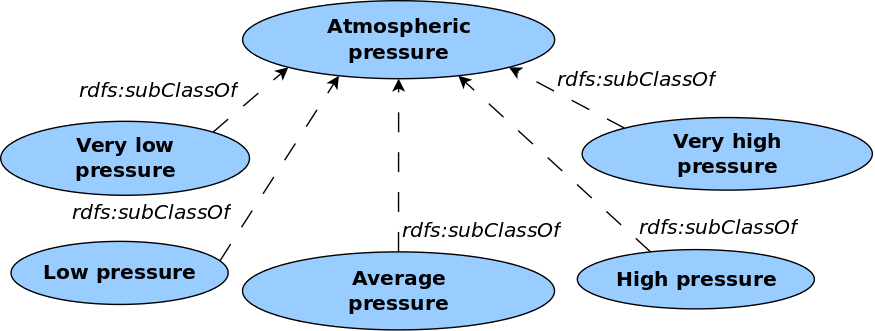
\includegraphics[width=.8\textwidth]{figures/diagrams/atmospheric-pressure.png}
  \caption{Concept-classification tree for \Egls{atmospheric pressure}}
  \label{fig:tree_atmospheric_pressure}
\end{figure}

\begin{figure}
  \centering
  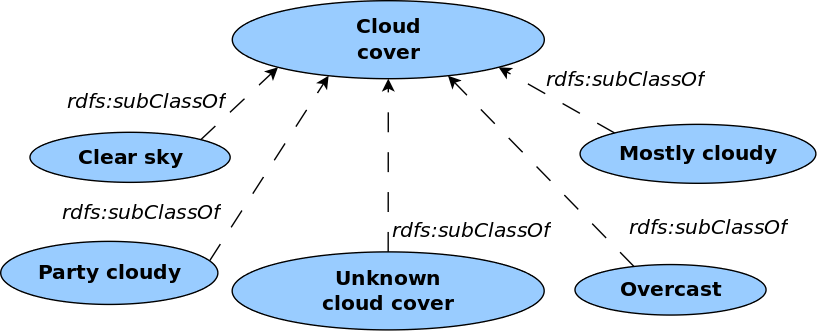
\includegraphics[width=.8\textwidth]{figures/diagrams/cloud-cover.png}
  \caption{Concept-classification tree for \Egls{cloud cover}}
  \label{fig:tree_cloud_cover}
\end{figure}

\begin{figure}
  \centering
  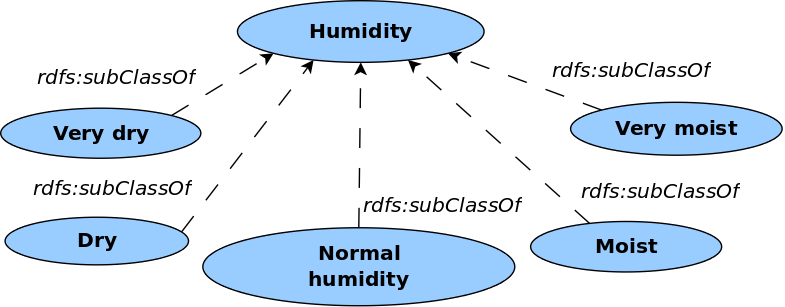
\includegraphics[width=.8\textwidth]{figures/diagrams/humidity.png}
  \caption{Concept-classification tree for \Egls{humidity}}
  \label{fig:tree_humidity}
\end{figure}

\begin{figure}
  \centering
  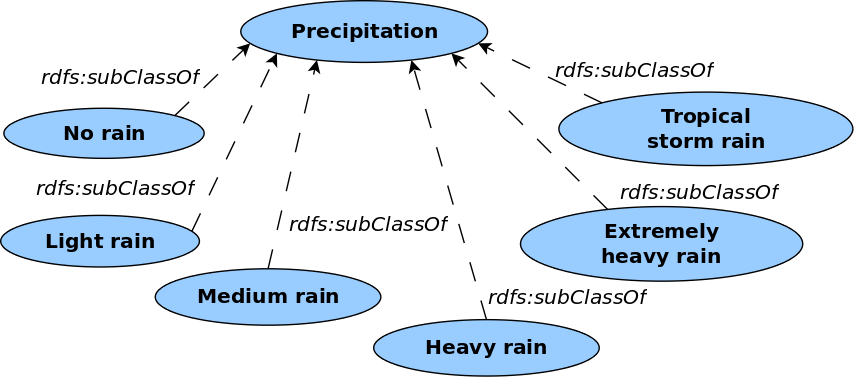
\includegraphics[width=.8\textwidth]{figures/diagrams/precipitation.png}
  \caption{Concept-classification tree for \Egls{precipitation}}
  \label{fig:tree_precipitation}
\end{figure}

\begin{figure}
  \centering
  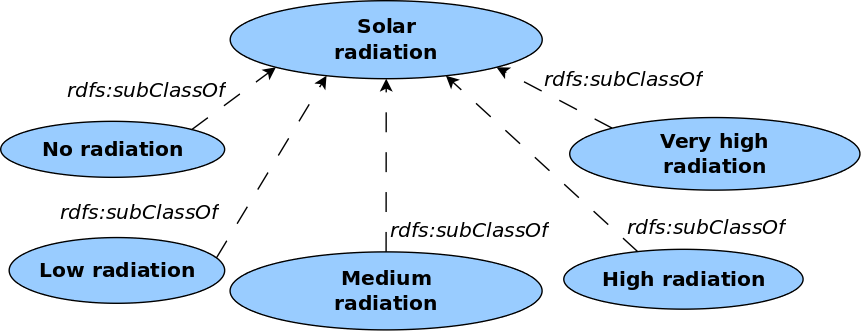
\includegraphics[width=.8\textwidth]{figures/diagrams/solar-radiation.png}
  \caption{Concept-classification tree for \Egls{solar radiation}}
  \label{fig:tree_solar_radiation}
\end{figure}

\begin{figure}
  \centering
  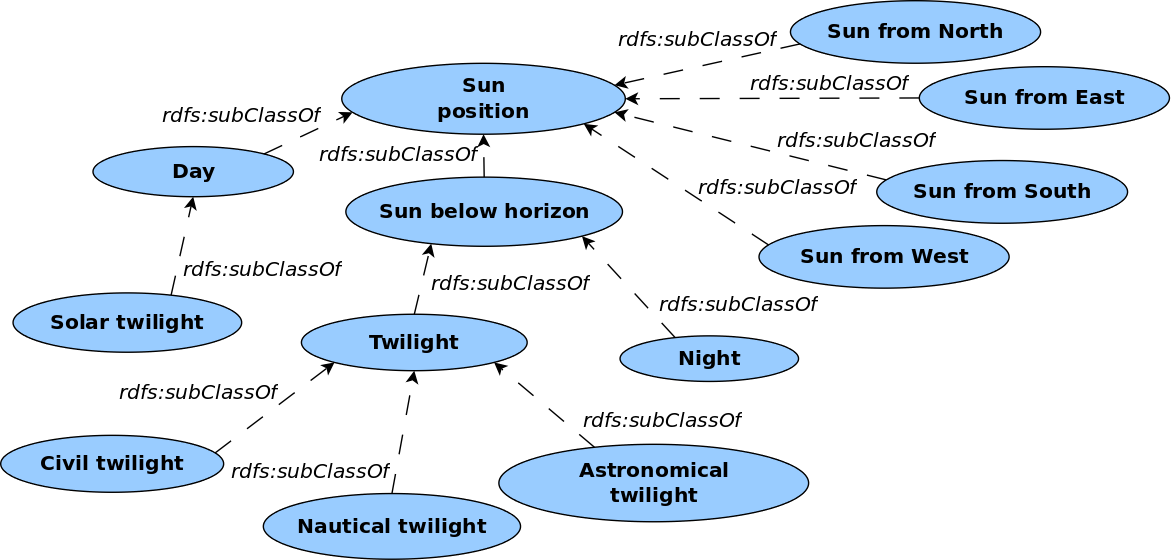
\includegraphics[width=.8\textwidth]{figures/diagrams/sun-position.png}
  \caption{Concept-classification tree for \Egls{sun position}}
  \label{fig:tree_sun_position}
\end{figure}

\begin{figure}
  \centering
  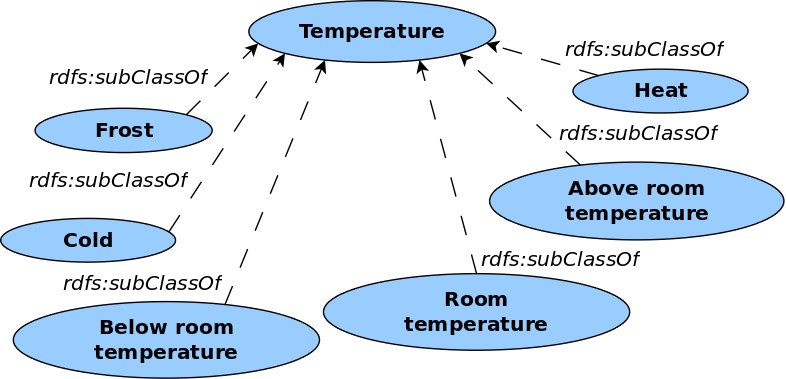
\includegraphics[width=.8\textwidth]{figures/diagrams/temperature.png}
  \caption{Concept-classification tree for \Egls{temperature}}
  \label{fig:tree_temperature}
\end{figure}

\begin{figure}
  \centering
  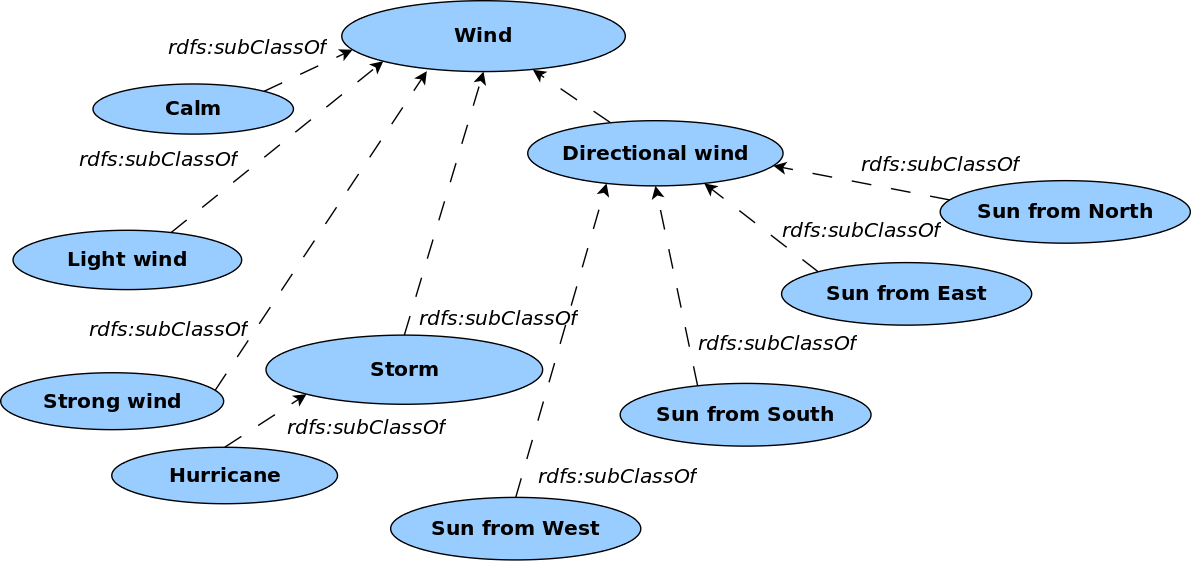
\includegraphics[width=\textwidth]{figures/diagrams/wind.png}
  \caption{Concept-classification tree for \Egls{wind}}
  \label{fig:tree_wind}
\end{figure}

A \Egls{weather report} has two attributes that define its main characteristics: \egls{has start time} and \egls{has source}. As discussed in section~\ref{sec:ontology_glossary}, a number of sub-concepts is defined in order to reflect different values of these two attributes. The resulting concept-classification tree is shown in figure~\ref{fig:tree_weather_report}.

\begin{figure}
  \centering
  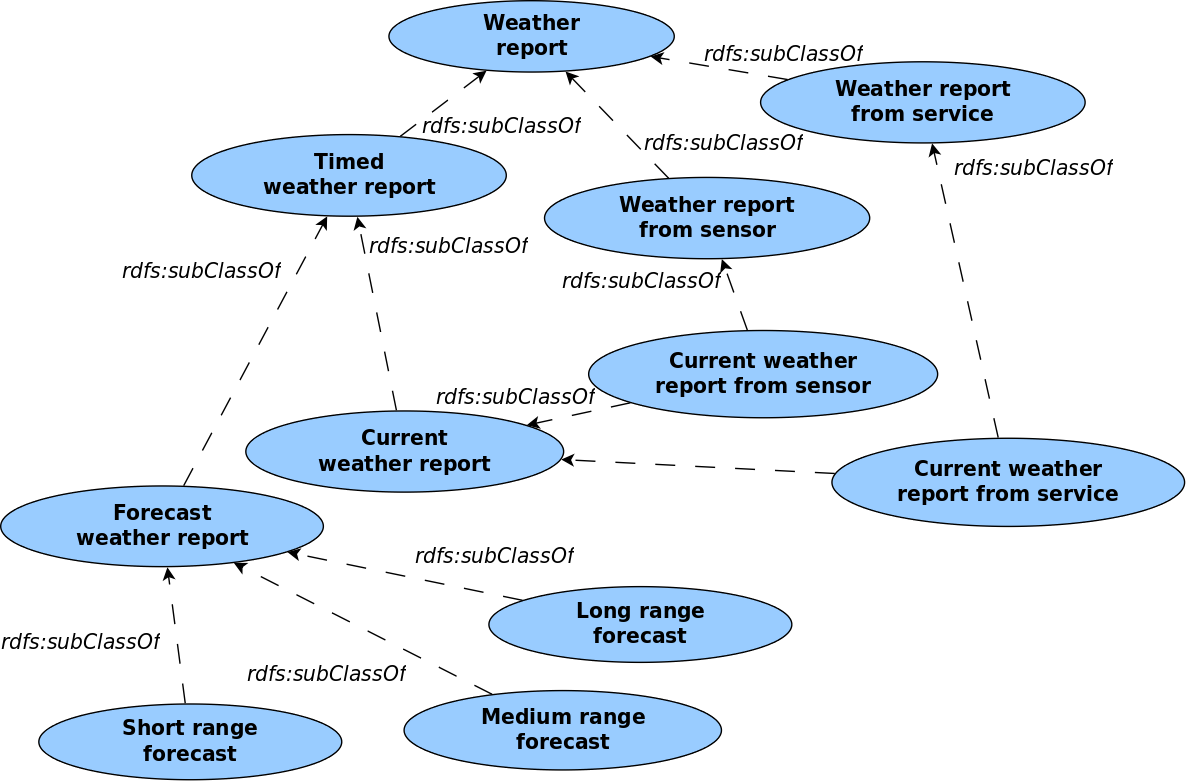
\includegraphics[width=\textwidth]{figures/diagrams/weather-report.png}
  \caption{Concept-classification tree for \Egls{weather report}}
  \label{fig:tree_weather_report}
\end{figure}

The concepts \Egls{short range weather report}, \Egls{medium range weather report} and \Egls{long range weather report} each do have sub-concepts which have been omitted from the above diagram for clarity. These sub-concepts are:
\begin{itemize}
  \item \Egls{short range weather report}: \emph{Forecast 1 hour weather report}, \emph{Forecast 2 hours weather report} and \emph{Forecast 3 hours weather report} for weather reports describing the weather in one, two and three hours, respectively.
  \item \Egls{medium range weather report}: \emph{Forecast 6 hour weather report} and \emph{Forecast 9 hours weather report} for weather reports describing the weather in 6 and 9 hours, respectively.
  \item \Egls{long range weather report}: \emph{Forecast 12 hour weather report}, \emph{Forecast 15 hours weather report}, \emph{Forecast 18 hours weather report}, \emph{Forecast 21 hours weather report} and \emph{Forecast 24 hours weather report} for weather reports describing the weather in 12, 15, 18, 21 and 24 hours, respectively.
\end{itemize}

A \Egls{weather source} can either be a \Egls{sensor source} or a \Egls{service source} (see figure~\ref{fig:tree_weather_source}).

\begin{figure}
  \centering
  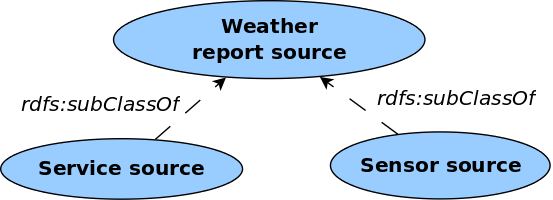
\includegraphics[width=.5\textwidth]{figures/diagrams/weather-report-source.png}
  \caption{Concept-classification tree for \Egls{weather source}}
  \label{fig:tree_weather_source}
\end{figure}

A \Egls{weather state} represents the set of weather phenomena that belong to a certain \Egls{weather report}. In order to emphasise certain combinations of instances of \Egls{weather phenomenon} being linked to the same instance of \Egls{weather state}, several sub-concepts of \Egls{weather state} are introduced (see figure~\ref{fig:tree_weather_state}): % TODO mention concepts and add them to the glossary

\begin{figure}
  \centering
  % TODO diagram is incomplete
  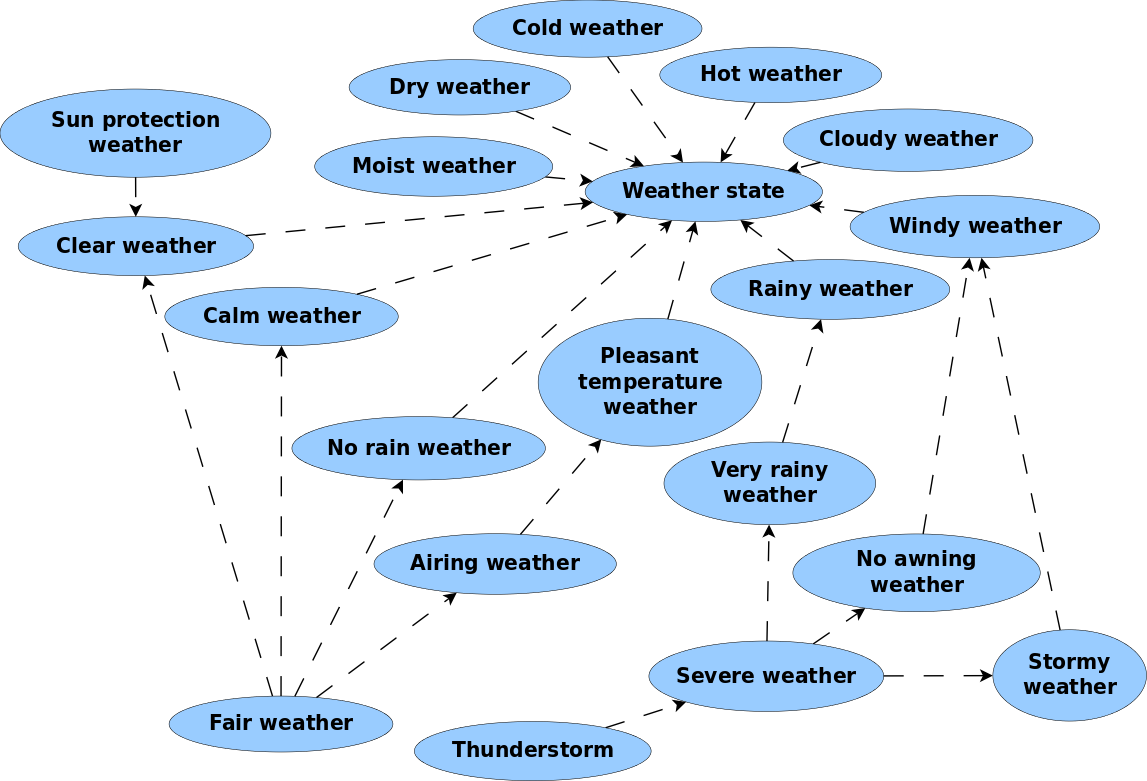
\includegraphics[width=.3\textwidth]{figures/diagrams/weather-state.png}
  \caption{Concept-classification tree for \Egls{weather state}}
  \label{fig:tree_weather_state}
\end{figure}

\subsection{Binary relations diagram}
\label{sec:binary_relations_diagram}

The purpose of a \emph{Binary relations diagram} is to present all binary relations between concepts in the ontology (see figure~\ref{fig:binary_relations}).

% TODO add previous/next weather state
\begin{figure}
  \centering
  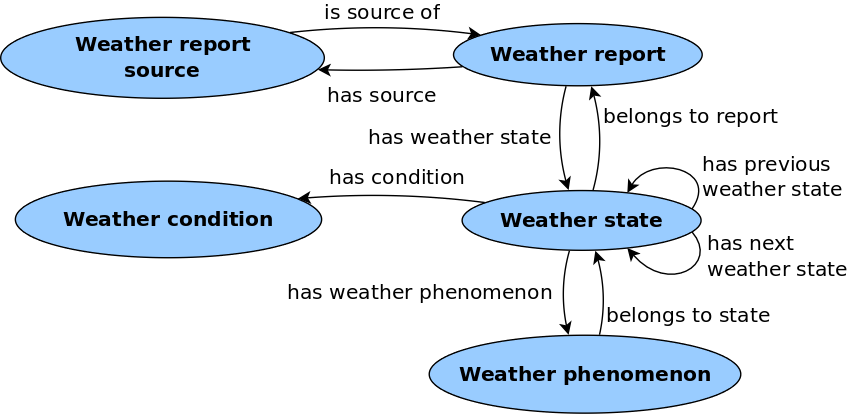
\includegraphics[width=.8\textwidth]{figures/diagrams/binary-relations.png}
  \caption{Binary relations diagram of \thinkhomeweather}
  \label{fig:binary_relations}
\end{figure}

\subsection{Concept dictionaries}

A \emph{Concept dictionary} lists all concepts together with their names, instances, class attributes, instance attributes and relations. For the sake of clarity, this table is split up into several tables, one for each of the concept-classification trees in section~\ref{sec:concept_classification_trees}.

In the following tables, sub-concepts having the same instances, class attributes, instance attributes and relations as their super-concepts are omitted. Furthermore, any columns that are not filled with any content in any row are omitted.

\subsubsection{Weather condition}

\begin{longtable}{|p{.2\textwidth}|p{.5\textwidth}|p{.2\textwidth}|}
  \hline
  \textbf{Name} & \textbf{Instances} & \textbf{Relations} \\
  \hline\hline
  \Egls{weather condition} & \emph{cloud}, \emph{fog}, \emph{partly cloudy}, \emph{mostly cloudy}, \emph{rain}, \emph{sleet}, \emph{snow}, \emph{sun}, \emph{thunder} & \egls{has condition} \\
  \hline
\end{longtable}

\subsubsection{Weather phenomenon}

\begin{longtable}{|p{.25\textwidth}|p{.3\textwidth}|p{.35\textwidth}|}
  \hline
  \textbf{Name} & \textbf{Instance attributes} & \textbf{Relations} \\
  \hline
  \Egls{atmospheric pressure} & \egls{has pressure value} & \egls{belongs to state},\newline \egls{has weather phenomenon} \\
  \hline
  \Egls{dew point} & \egls{has dew point value} & \egls{belongs to state},\newline \egls{has weather phenomenon} \\
  \hline
  \Egls{humidity} & \egls{has humidity value} & \egls{belongs to state},\newline \egls{has weather phenomenon} \\
  \hline
  \Egls{precipitation} & \egls{has precipitation intensity},\newline \egls{has precipitation probability} & \egls{belongs to state},\newline \egls{has weather phenomenon} \\
  \hline
  \Egls{sun position} & \egls{has sun elevation angle},\newline \egls{has sun direction} & \egls{belongs to state},\newline \egls{has weather phenomenon} \\
  \hline
  \Egls{solar radiation} & \egls{has solar radiation value} & \egls{belongs to state},\newline \egls{has weather phenomenon} \\
  \hline
  \Egls{temperature} & \egls{has temperature value} & \egls{belongs to state},\newline \egls{has weather phenomenon} \\
  \hline
  \Egls{weather phenomenon} & - & \egls{belongs to state},\newline \egls{has weather phenomenon} \\
  \hline
  \Egls{wind} & \egls{has wind speed},\newline \egls{has wind direction} & \egls{belongs to state},\newline \egls{has weather phenomenon} \\
  \hline
\end{longtable}

\subsubsection{Weather report}

\begin{longtable}{|p{.2\textwidth}|p{.3\textwidth}|p{0.35\textwidth}|}
  \hline
  \textbf{Name} & \textbf{Instance\newline attributes} & \textbf{Relations} \\
  \hline\hline
  \Egls{weather report} & \Egls{has priority}, \Egls{location}, \newline \Egls{has start time}, \Egls{has end time},\newline \Egls{has observation time}  & \egls{has source}, \egls{is source of},\newline \egls{has weather state}, \newline \egls{belongs to weather report} \\
  \hline
\end{longtable}

\subsubsection{Weather state}

% TODO sub-concepts
\begin{longtable}{|p{0.167\textwidth}|p{0.167\textwidth}|p{0.167\textwidth}|p{0.167\textwidth}|p{0.167\textwidth}|}
  \hline
  \textbf{Name} & \textbf{Instances} & \textbf{Class\newline attributes} & \textbf{Instance\newline attributes} & \textbf{Relations} \\
  \hline\hline
  \Egls{weather state} & - & - & - & \egls{has condition},\newline \egls{belongs to weather report},\newline \egls{has weather state},\newline \egls{belongs to state},\newline \egls{has weather phenomenon}\\
  \hline
\end{longtable}

\subsubsection{Weather source}

\begin{longtable}{|p{0.3\textwidth}|p{0.6\textwidth}|}
  \hline
  \textbf{Name} & \textbf{Relations} \\
  \hline\hline
  \Egls{weather source} & \egls{is source of}, \egls{has source} \\
  \hline
  \Egls{sensor source} & \egls{is source of}, \egls{has source} \\
  \hline
  \Egls{service source} & \egls{is source of}, \egls{has source} \\
  \hline
\end{longtable}

\subsection{Binary relations table}

The \emph{Binary relation table} specifies all relations from section~\ref{sec:binary_relations_diagram} in detail. This includes the relations' names, their source and target concepts, their maximum source cardinalities and their inverse relations, if any.

\begin{longtable}{|p{.167\textwidth}|p{.167\textwidth}|p{.167\textwidth}|p{.167\textwidth}|p{.167\textwidth}|}
  \hline
  \textbf{Name} & \textbf{Source\newline concept} & \textbf{Target\newline concept} & \textbf{Maximum\newline source\newline cardinality} & \textbf{Inverse\newline relation} \\
  \hline\hline
  \egls{belongs to state} & \Egls{weather phenomenon} & \Egls{weather state} & $1$ & \egls{has weather phenomenon} \\
  \hline
  \egls{belongs to weather report} & \Egls{weather state} & \Egls{weather report} & $1$ & \egls{has weather state} \\
  \hline
  \egls{has condition} & \Egls{weather state} & \Egls{weather condition} & $N$ & - \\
  \hline
  \egls{has next weather state} & \Egls{weather report} & \Egls{weather report} & $1$ & \egls{has previous weather state} \\
  \hline
  \egls{has previous weather state} & \Egls{weather report} & \Egls{weather report} & $1$ & \egls{has next weather state} \\
  \hline
  \egls{has source} & \Egls{weather report} & \Egls{weather source} & $1$ & \egls{is source of} \\
  \hline
  \egls{has weather phenomenon} & \Egls{weather state} & \Egls{weather phenomenon} & $N$ & \egls{belongs to state} \\
  \hline
  \egls{has weather state} & \Egls{weather report} & \Egls{weather state} & $1$ & \egls{belongs to weather report} \\
  \hline
  \egls{is source of} & \Egls{weather source} & \Egls{weather report} & $N$ & \egls{has source} \\
  \hline
\end{longtable}

\subsection{Instance attribute tables}
\label{subsec:instance_attribute_tables}

% TODO add instant, interval and temporalentity to glossary

% TODO description of what is going on here
% TODO

The data types \emph{xsd:integer} and \emph{xsd:decimal} refer to the types defined in \emph{XML Schema}\cite{xml-schema-datatypes}. \emph{time:instant} and \emph{time:interval} refer to the types \emph{Instant} and \emph{Interval} from the \emph{OWL-Time}  ontology\cite{owl-time}.

% TODO remove times and location from here as they are not instance attributes
\begin{longtable}{|p{0.15\textwidth}|p{0.15\textwidth}|p{0.15\textwidth}|p{0.15\textwidth}|p{0.15\textwidth}|p{0.15\textwidth}|}
  \hline
  \textbf{Attribute name} & \textbf{Concept name} & \textbf{Value type} & \textbf{Value range} & \textbf{Unit} & \textbf{Cardinality} (min, max)\\
  \hline\hline
  \egls{alt} & \Egls{location} & \emph{xsd:decimal} & \emph{any values allowed} & \metre & $(1, 1)$ \\
  \hline
  \egls{has cloud altitude} & \Egls{cloud cover} & \emph{xsd:decimal} & \emph{any values allowed} & \metre & $(1, 1)$ \\
  \hline
  \egls{has cloud cover} & \Egls{cloud cover} & \emph{xsd:integer} & $[0, 9]$ & \Egls{okta} & $(1, 1)$ \\
  \hline
  \egls{has dew point value} & \Egls{dew point} & \emph{xsd:decimal} & \emph{any values allowed} & \celsius & $(1, 1)$ \\
  \hline
  \egls{has end time} & \Egls{weather report} & \emph{time:interval} & \emph{any values allowed} & - & $(1, 1)$ \\
  \hline
  \egls{has humidity value} & \Egls{humidity} & \emph{xsd:decimal} & $[0, 1]$ & - & $(1, 1)$ \\
  \hline
  \egls{lat} & \Egls{location} & \emph{xsd:decimal} & $[-90, 90]$ & \degree\space(degrees) & $(1, 1)$ \\
  \hline
  \egls{long} & \Egls{location} & \emph{xsd:decimal} & $[-180, 180]$ & \degree\space(degrees) & $(1, 1)$ \\
  \hline
  \egls{observation time} & \Egls{weather report} & \emph{time:instant} & \emph{any values allowed} & - & $(1, 1)$ \\
  \hline
  \egls{has precipitation intensity} & \Egls{precipitation} & \emph{xsd:decimal} & $[0, \infty)$ & \milli\metre\per\hour & $(1, 1)$ \\
  \hline
  \egls{has precipitation probability} & \Egls{precipitation} & \emph{xsd:decimal} & $[0, 1]$ & - & $(1, 1)$ \\
  \hline
  \egls{has pressure value} & \Egls{atmospheric pressure} & \emph{xsd:decimal} & $[0, \infty)$ & \hecto\pascal & $(1, 1)$ \\
  \hline
  \egls{has start time} & \Egls{weather report} & \emph{time:interval} & \emph{any values allowed} & - & $(1, 1)$ \\
  \hline
  \egls{has solar radiation value} & \Egls{solar radiation} & \emph{time:decimal} & $[0, \infty)$ & \watt\per\squaren\meter & $(1, 1)$ \\
  \hline
  \egls{has sun direction} & \Egls{sun position} & \emph{xsd:decimal} & $[0, 360)$ & \degree\space(degrees) & $(1, 1)$ \\
  \hline
  \egls{has sun elevation angle} & \Egls{sun position} & \emph{xsd:decimal} & $[-90, 90]$ & \degree\space(degrees) & $(1, 1)$ \\
  \hline
  \egls{has temperature value} & \Egls{temperature} & \emph{xsd:decimal} & \emph{any values allowed} & \celsius & $(1, 1)$ \\
  \hline
  \egls{has wind direction} & \Egls{wind} & \emph{xsd:decimal} & $[0, 360)$ & \degree\space(degrees) & $(1, 1)$ \\
  \hline
  \egls{has wind speed} & \Egls{wind} & \emph{xsd:decimal} & $[0, \infty)$ & \metre\per\second & $(1, 1)$ \\
  \hline
\end{longtable}

\subsection{Class attribute tables}

% TODO ?
The ontology does not contain any class attributes, hence there is no table describing the class attributes' properties.

\subsection{Logical axioms tables} % TODO formal axioms

% TODO ?
There are no logical axioms that will be encoded into the ontology, hence there is no table describing logical axioms.

% TODO missing section: constants?

% TODO are those actually class attributes?
\subsection{Formula tables} % TODO rules?

Many concepts within the \thinkhomeweather ontology define themselves to be specializations of other concepts. E.g. the concepts \emph{Very low pressure}, \emph{Low pressure}, \emph{Normal pressure}, \emph{High pressure} and \emph{Very high pressure} are all sub-concepts of \emph{Atmospheric pressure}. They all differ by the value of the instance attribute \emph{has pressure value} that every instance of \emph{Atmospheric pressure} has.

In the Glossary of Terms, \emph{Normal pressure} is defined to be an instance of \emph{Atmospheric pressure} having a value of at least 1008 and at most 1018 hPa to be assigned via \emph{has pressure value}. One could write this rule in the following manner:

% TODO description
% TODO format, no page breaks within
\begin{verbatim}
if Atmospheric pressure(?X)
  and has pressure value(?X, ?Y)
  and ?Y >= 1008 and ?Y <= 1018
then Normal pressure(?X)
\end{verbatim}

As a long list of such rules becomes apparently confusing, the relevant information is summarized in a table. In the case of the super-concept \emph{Atmospheric pressure}, this table has three columns: One that takes the name of the super-concept, one takes the name of the sub-concept and one the value range of the instance attribute \emph{has pressure value}. For the sub-concept \emph{Normal pressure}, this table evolves:

% TODO 
\begin{longtable}{|p{0.25\textwidth}|p{0.25\textwidth}|p{0.25\textwidth}|}
  \hline
  \textbf{Super-concept} & \textbf{Sub-concept} & \textbf{has pressure value} \\
  \hline\hline
  Atmospheric pressure & Normal pressure & $[1008, 1018)$ \\
  \hline
\end{longtable}

There are sub-concepts defined by restrictions on more than one instance attribute. In such a case, columns are added to the respective table as needed. For instance, sub-concepts of \emph{Wind} have restrictions on both the instance attribute \emph{has wind speed} and on the instance attribute \emph{has wind direction}. In that case, the table has four columns: Super-concept, sub-concept, \emph{has wind speed} and \emph{has wind direction}.

If there is more than one row for a certain sub-concept, these rows specify alternatives: The instance of the super-concept is an instance of the sub-concept, if any of the restrictions in the respective rows holds.

If the value of an instance attribute is not significant for an instance of the super-concept being also an instance of the sub-concept, this is indicated by a dash (-).

% TODO reference?
In the following sections, for each concept-classification tree shown above, the respective table is given.

\subsubsection{Atmospheric pressure}

\begin{longtable}{|p{0.25\textwidth}|p{0.25\textwidth}|p{0.25\textwidth}|}
  \hline
  \textbf{Super-concept} & \textbf{Sub-concept} & \textbf{has pressure value} \\
  \hline\hline
  Atmospheric pressure & Very low pressure & $< 998$ \\
  \hline
  Atmospheric pressure & Low pressure & $[998, 1008)$ \\
  \hline
  Atmospheric pressure & Normal pressure & $[1008, 1018)$ \\
  \hline
  Atmospheric pressure & High pressure & $[1018, 1028)$ \\
  \hline
  Atmospheric pressure & Very high pressure & $\geq 1028$ \\
  \hline
\end{longtable}

\subsubsection{Cloud cover}

\begin{longtable}{|p{0.25\textwidth}|p{0.25\textwidth}|p{0.25\textwidth}|}
  \hline
  \textbf{Super-concept} & \textbf{Sub-concept} & \textbf{has cloud cover} \\
  \hline\hline
  Cloud cover & Clear sky & 0 \\
  \hline
  Cloud cover & Partly cloudy & 1, 2, 3, 4 \\
  \hline
  Cloud cover & Mostly cloudy & 5, 6, 7 \\
  \hline
  Cloud cover & Overcast & 8 \\
  \hline
  Cloud cover & Unknown cloud cover & 9 \\
  \hline
\end{longtable}

\subsubsection{Humidity}

\begin{longtable}{|p{0.25\textwidth}|p{0.25\textwidth}|p{0.25\textwidth}|}
  \hline
  \textbf{Super-concept} & \textbf{Sub-concept} & \textbf{has humidity value} \\
  \hline\hline
  Humidity & Very dry & $< 0.3$ \\
  \hline
  Humidity & Dry & $[0.3, 0.4)$ \\
  \hline
  Humidity & Normal humidity & $[0.4, 0.7]$ \\
  \hline
  Humidity & Moist & $(0.7, 0.8]$ \\
  \hline
  Humidity & Very moist & $> 0.8$ \\
  \hline
\end{longtable}

\subsubsection{Precipitation}

\begin{longtable}{|p{0.2\textwidth}|p{0.2\textwidth}|p{0.2\textwidth}|p{0.2\textwidth}|}
  \hline
  \textbf{Super-concept} & \textbf{Sub-concept} & \textbf{has precipitation\newline probability} & \textbf{has precipitation\newline intensity} \\
  \hline\hline
  Precipitation & No rain & $0$ & - \\
  \hline
  Precipitation & No rain & - & $0$ \\
  \hline
  Precipitation & Light rain & $(0, 1]$ & $(0, 5]$ \\
  \hline
  Precipitation & Medium rain & $(0, 1]$ & $(5, 20]$ \\
  \hline
  Precipitation & Heavy rain & $(0, 1]$ & $(20, 50]$ \\
  \hline
  Precipitation & Extremely heavy rain & $(0, 1]$ & $(50, 100]$ \\
  \hline
  Precipitation & Tropical storm rain & $(0, 1]$ & $> 100$ \\
  \hline
\end{longtable}

\subsubsection{Solar radiation}

\begin{longtable}{|p{0.25\textwidth}|p{0.25\textwidth}|p{0.25\textwidth}|}
  \hline
  \textbf{Super-concept} & \textbf{Sub-concept} & \textbf{has solar\newline radiation value} \\
  \hline\hline
  Solar radiation & No radiation & $0$ \\
  \hline
  Solar radiation & Low radiation & $(0, 250)$ \\
  \hline
  Solar radiation & Medium radiation & $[250, 500)$ \\
  \hline
  Solar radiation & High radiation & $[500, 750)$ \\
  \hline
  Solar radiation & Very high radiation & $\geq 750$ \\
  \hline
\end{longtable}

\subsubsection{Sun position}

\begin{longtable}{|p{0.2\textwidth}|p{0.2\textwidth}|p{0.2\textwidth}|p{0.2\textwidth}|}
  \hline
  \textbf{Super-concept} & \textbf{Sub-concept} & \textbf{has sun\newline direction} & \textbf{has sun\newline elevation angle} \\
  \hline\hline
  Sun position & Sun from north & $(0, 45]$ & - \\
  \hline
  Sun position & Sun from north & $(315, 360)$ & - \\
  \hline
  Sun position & Sun from east & $(45, 135]$ & - \\
  \hline
  Sun position & Sun from south & $(135, 225]$ & - \\
  \hline
  Sun position & Sun from west & $(225, 315]$ & - \\
  \hline
  Sun position & Day & - & $[0, 90]$ \\
  \hline
  Sun position & Solar twilight & - & $[0, 6)$ \\
  \hline
  Sun position & Sun below horizon & - & $[-90, 0)$ \\
  \hline
  Sun position & Twilight & - & $[-18, 0)$ \\
  \hline
  Sun position & Civil twilight & - & $[-6, 0)$ \\
  \hline
  Sun position & Nautical twilight & - & $[-12, -6)$ \\
  \hline
  Sun position & Astronomical twilight & - & $[-18, -12)$ \\
  \hline
  Sun position & Night & - & $[-90, -18)$ \\
  \hline
\end{longtable}

\subsubsection{Temperature}

\begin{longtable}{|p{0.25\textwidth}|p{0.25\textwidth}|p{0.25\textwidth}|}
  \hline
  \textbf{Super-concept} & \textbf{Sub-concept} & \textbf{has temperature\newline value} \\
  \hline\hline
  Temperature & Frost & $< 0$ \\
  \hline
  Temperature & Cold & $[0, 10)$ \\
  \hline
  Temperature & Below room temperature & $[10, 20)$ \\
  \hline
  Temperature & Room temperature & $[20, 25]$ \\
  \hline
  Temperature & Above room temperature & $(25, 30]$ \\
  \hline
  Temperature & Heat & $> 30$ \\
  \hline
\end{longtable}

\subsubsection{Wind}

\begin{longtable}{|p{0.2\textwidth}|p{0.2\textwidth}|p{0.2\textwidth}|p{0.2\textwidth}|}
  \hline
  \textbf{Super-concept} & \textbf{Sub-concept} & \textbf{has wind\newline speed} & \textbf{has wind\newline direction} \\
  \hline\hline
  Wind & Directional wind & - & $[0, 360)$ \\
  \hline
  Wind & North wind & - & $[0, 45)$ \\
  \hline
  Wind & North wind & - & $(315, 360)$ \\
  \hline
  Wind & East wind & - & $[45, 135)$ \\
  \hline
  Wind & South wind & - & $[135, 225)$ \\
  \hline
  Wind & West wind & - & $[225, 315)$ \\
  \hline
  Wind & Calm & $[0, 1)$ & - \\
  \hline
  Wind & Light wind & $[1, 10)$ & - \\
  \hline
  Wind & Strong wind & $[10, 20)$ & - \\
  \hline
  Wind & Storm & $\geq 20$ & - \\
  \hline
  Wind & Hurricane & $\geq 32$ & - \\
  \hline
\end{longtable}

\subsubsection{Weather report}

\begin{longtable}{|p{0.2\textwidth}|p{0.2\textwidth}|p{0.2\textwidth}|p{0.2\textwidth}|}
  \hline
  \textbf{Super-concept} & \textbf{Sub-concept} & \textbf{has start time} & \textbf{has source} \\
  \hline\hline
  Weather report & Current weather report & $0$ & - \\
  \hline
  Weather report & Forecast weather report & $> 0$ & - \\
  \hline
  Weather report & Forecast 1 hour weather report & $1$ & - \\
  \hline
  Weather report & Forecast 2 hours weather report & $2$ & - \\
  \hline
  Weather report & Forecast 3 hours weather report & $3$ & - \\
  \hline
  Weather report & Forecast 6 hours weather report & $6$ & - \\
  \hline
  Weather report & Forecast 9 hours weather report & $9$ & - \\
  \hline
  Weather report & Forecast 12 hours weather report & $12$ & - \\
  \hline
  Weather report & Forecast 15 hours weather report & $15$ & - \\
  \hline
  Weather report & Forecast 18 hours weather report & $18$ & - \\
  \hline
  Weather report & Forecast 21 hours weather report & $21$ & - \\
  \hline
  Weather report & Forecast 24 hours weather report & $24$ & - \\
  \hline
  Weather report & Short range weather report & $(0, 3]$ & - \\
  \hline
  Weather report & Medium range weather report & $(3, 12)$ & - \\
  \hline
  Weather report & Long range weather report & $\geq 12$ & - \\
  \hline
  Weather report & Weather report from sensor & - & \emph{any instance of Weather sensor} \\
  \hline
  Weather report & Weather report from service & - & \emph{any instance of Weather service} \\
  \hline
  Weather report & Current weather report from sensor & $0$ & \emph{any instance of Weather sensor} \\
  \hline
  Weather report & Current weather report from service & $0$ & \emph{any instance of Weather service} \\
  \hline
\end{longtable}

% TODO sub-concepts of weather state

\subsection{Instance tables}

% TODO description of what is going on here
% TODO
\begin{longtable}{|p{0.2\textwidth}|p{0.2\textwidth}|p{0.2\textwidth}|p{0.2\textwidth}|}
  \hline
  \textbf{Instance name} & \textbf{Concept name} & \textbf{Attribute} & \textbf{Values} \\
  \hline\hline
  Cloud & Weather condition & - & - \\
  \hline
  Fog & Weather condition & - & - \\
  \hline
  Partly cloudy & Weather condition & - & - \\
  \hline
  Mostly cloudy & Weather condition & - & - \\
  \hline
  Rain & Weather condition & - & - \\
  \hline
  Sleet & Weather condition & - & - \\
  \hline
  Snow & Weather condition & - & - \\
  \hline
  Sun & Weather condition & - & - \\
  \hline
  Thunder & Weather condition & - & - \\
  \hline
\end{longtable}

\section{Integration}
\label{sec:integration}

One of the goals of the \thinkhomeweather ontology is to keep an eye on existing ontologies to be re-used. While analyzing the problem domain, it quickly became clear that there are four areas where already existing ontologies could be reused: Location data, measuremenr units, date/time specifications and weather concepts. Chapter \ref{ch:existing_work} already sheds some light on existing ontologies around the domain of weather data. In this section, the ontologies being short-listed for reuse within \thinkhomeweather are summarized.

% TODO reference: website, WGS84
For location data, the W3C Semantic Web Interest Group offers a \emph{Basic Geo (WGS84 lat/long) Vocabulary}. It introduces a concept called \emph{Spatial thing} that can have \emph{latitude}, \emph{longitude} and \emph{altitude} according to the WGS 84 geodetic reference system. However, the vocabulary contains some data properties that are incorrectly defined as annotation property. This shortcoming needs to be overriden in any ontology that uses this vocabulary.

% TODO reference SWEET
NASA's SWEET ontology offers a wide range of concepts, attributes and individuals for environmental and atmospherical phenomena, including all units that may be used within a weather data ontology. SWEET is designed in a highly modular manner. Units can be found in a single OWL file. However, importing one of SWEET's OWL files into an ontology entails the import of a large number of other OWL files. As this makes any simple ontology using SWEET hard to handle, reusing SWEET is not an option.

Besides SWEET, there is no ontology containing weather concepts that has been determined to be appropriate for use within the \thinkhomeweather ontology. Hence, \thinkhomeweather defines its own weather concepts.

% TODO reference: http://forge.morfeo-project.org/wiki_en/index.php/Units_of_measurement_ontology
% TODO reference: http://idi.fundacionctic.org/muo/muo-vocab.html
The \emph{Measurement Units Ontology} is a simple and light-weight approach to enrich measurement values with appropriate units. Some of the most important units are pre-defined, all others can easily be added. The \emph{Measurement Units Ontology} (MUO) is still work in progress. However, it is not expected that it might change heavily in the future. Everything that will be reused by other ontologies will remain unchanged. Hence, MUO can be imported into any ontology without problems.

Besides the \emph{Measurement Units Ontology}, several other ontologies have been examined, but all of them came with shortcomings that led to the decision not to use them in the \thinkhomeweather ontology. These ontologies are:
\begin{itemize}
  \item \textbf{SWEET:} Besides concepts, attributes and individuals for atmospherical phenomena, SWEET also comes with support for literals more precisely specified by units. However, as mentioned above importing any part of SWEET entails the import of a large number of OWL files that makes handling a ontology using SWEET difficult. Hence, SWEET is not used for introducing units into the \thinkhomeweather ontology.
  \item \textbf{QUDT:} \emph{QUDT}, a set of ontologies for \emph{Quantities, Units, Dimensions and Data Types in OWL and XML}, is a promising approach for adding support for units to an OWL ontology. However, \emph{QUDT} does not work in \protege together with the Pellet reasoner. Using \emph{QUDT} would require several changes to the OWL files. Hence, it cannot be used in the \thinkhomeweather ontology. % TODO reference http://www.qudt.org/
  \item \textbf{QUOMOS:} The \emph{OASIS Quantities and Units of Measure Ontology Standard} (\emph{QUOMOS}) aims at developing ``an ontology for quantities, systems of measurement units, and base dimensions for use across multiple industries''. However, at the time of writing, there is no release of any OWL ontology yet. % TODO reference https://www.oasis-open.org/committees/tc_home.php?wg_abbrev=quomos
  \item \textbf{OBO Foundry Initiative:} The \emph{OBO Foundry Initiative} is an initiative that aims at collecting ontologies for use in the biomedical domain. The list of \emph{The Open Biological and Biomedical Ontologies} (abbreviated by \emph{OBO}) includes an ontology for units of measurements. This ontology apparently covers most of the units that are used in the \thinkhomeweather ontology. However, it lacks any documentation and hence cannot be used in \thinkhomeweather. % TODO reference http://obofoundry.org/ and http://obofoundry.org/cgi-bin/detail.cgi?id=unit and http://code.google.com/p/unit-ontology/
\end{itemize}
Although the \emph{Measurement Units Ontology} has the shortcoming of making OWL reasoning clearly slower, it is the only ontology that has been determined to be usable in the \thinkhomeweather ontology flawlessly.

% TODO reference W3C consortium
% TODO reference W3C working draft definition
% TODO reference http://www.w3.org/TR/owl-time/
For specifying temporal properties, the W3C consortium offers a working draft of \emph{OWL-Time}, a \emph{Time Ontology in OWL}. It defines the concept called \emph{TemporalEntity} that can either be an \emph{Instant} or an \emph{Interval}. Using appropriate attributes, the properties of a \emph{TemporalEntity} are specified. Although \emph{OWL-Time} is in the state of a working draft since September 2006, the main concepts and attributes that will be reused by other ontologies are expected not to change in any way.

% TODO mention meta-ontology

Section \ref{sec:implementation} describes the reuse of the aforementioned ontologies within the \thinkhomeweather ontology in detail.

\section{Implementation}
\label{sec:implementation}

After exhaustive analysis and structurization in the previous sections, the step of implementing the ontology has become a straight-forward task.

% TODO reference OWL, Protege, Pellet
% TODO \emph{} for names
The \thinkhomeweather ontology is implemented in OWL using Protege 4.1 together with the Pellet OWL 2 Reasoner. Pellet includes Pellint, an ontology performance tool that uses a set of patterns to find possible performance problems in an OWL ontology. Pellint has been used for locating problems and led to a few improvements boosting reasoning performance.

To ensure that the reasoning of all sub-concepts of \emph{Weather phenomenon}, \emph{Weather state} and \emph{Weather report} works correctly, a JUnit is used. Every test case loads the \thinkhomeweather ontology using the \emph{Jena framework}, adds appropriate individuals and checks using the \emph{Pellet reasoner} if reasoning is performed in the desired manner.

\subsection{Imported ontologies}

During the implementation step, the ontologies listed in section \ref{sec:integration} need to be imported and integrated. Their use implies the application of certain patterns required by the ontologies.

% TODO reference OWL-Time
\emph{OWL-Time} defines the concept \emph{TemporalEntity} and its sub-concepts \emph{Instant} and \emph{Interval}. Although \emph{Start time} and \emph{End time} of a \emph{Weather report} are actually \emph{Instant}s (WHY?), these times are specified using \emph{Interval}s. The duration of such an interval represents the duration between the \emph{Observation time} of the \emph{Weather report} and the time that is to be expressed. This results in the structure shown in figure \ref{fig:owl_time1}. The duration is rounded to full hours. Hence, there are simple rules for defining concepts for a \emph{Weather report} for forecasts in an arbitrary number of hours.

\begin{figure}
  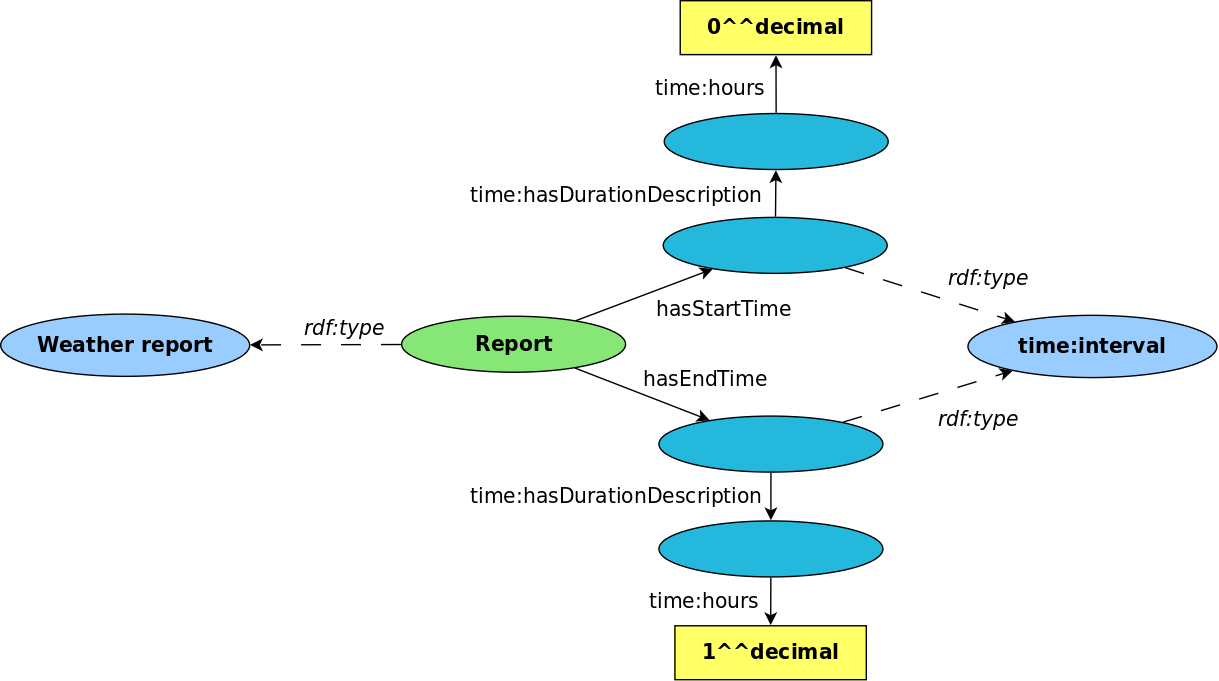
\includegraphics[width=\textwidth]{figures/diagrams/owl-time1.png}
  \caption{An instance of \emph{Current weather report} together with start time and end time.}
  \label{fig:owl_time1}
\end{figure}

The \emph{Observation time} of a \emph{Weather report} is specified using an \emph{Instant} as defined by \emph{OWL-time}. See figure \ref{fig:owl_time2} for the resulting structure.

% TODO figure 5.2: interval -> Interval
\begin{figure}
  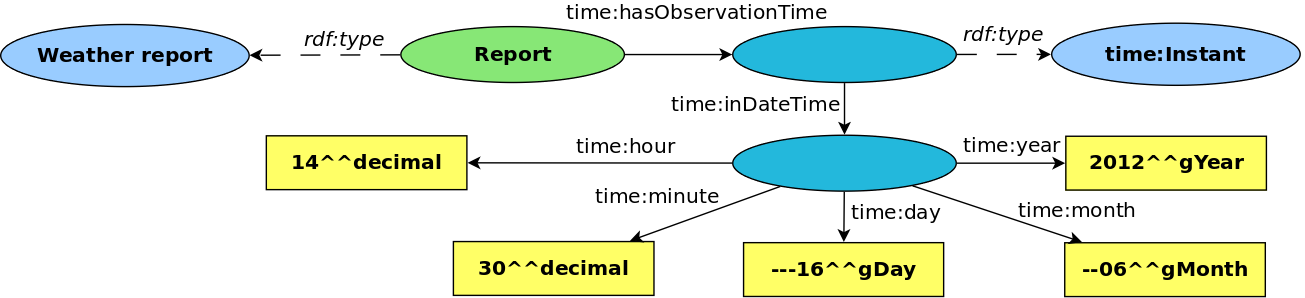
\includegraphics[width=\textwidth]{figures/diagrams/owl-time2.png}
  % TODO no line break inside the date string
  \caption{An instance of \emph{Weather report} together with its observation time (2012-06-16 14:30).}
  \label{fig:owl_time2}
\end{figure}

The \emph{Time Zone Ontology} that comes with \emph{OWL-Time} is not used by \thinkhomeweather. All times must be given in UTC.

% TODO reference unit ontology
All instances of \emph{Weather phenomenon} have one or more attributes specifying details about the weather element that is being represented (refer to section \ref{subsec:instance_attribute_tables} for details about these attributes). Each of these attributes assigns a numerical value to the \emph{Weather phenomenon}. To avoid confusion by the use of different units for one attribute (e.g. $^\circ$F and $^\circ$C for the \emph{Temperature value}), concepts, attributes and instances from the \emph{Measurement Units Ontology} (MUO) are re-used to add unit information. MUO forces the use of a certain pattern that is shown in figure . % TODO reference figure

% TODO reference WGS-84
The \emph{Basic Geo (WGS84 lat/long) Vocabulary} by the \emph{W3C Semantic Web Interest Group} defines the concept \emph{Point} together with the attributes \emph{lat} (latitude), \emph{long} (longitude) and \emph{alt} (altitude). Furthermore, the attribute \emph{location} offers the possibility of connecting a \emph{Point} to any instance of some concept. See figure \label{fig:wgs84} for the structure that results from this. % TODO reference figure

\begin{figure}
  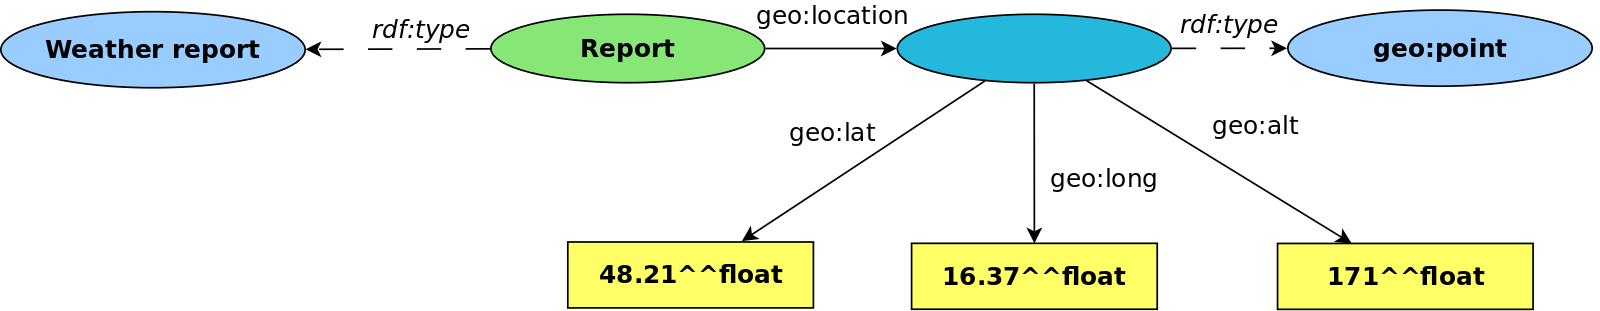
\includegraphics[width=\textwidth]{figures/diagrams/wgs84.png}
  \caption{An instance of \emph{Weather report} together with its location (Vienna, Austria: $48.21 ^{\circ} N$, $16.37 ^{\circ} E$, $171 m$ above MSL.}
  \label{fig:owl_time}
\end{figure}

% TODO document completed ontology thoroughly
\subsection{Naming conventions}

During the implementation of the \thinkhomeweather ontology, it is necessary to define strict naming conventions for concepts, individuals and attributes; some of these conventions have already been applied to previous steps of developing the ontology:

\begin{itemize}
  \item All concepts, instances and attributes share one namespace, regardless of capitalization; e.g. there is no pair of a concept and an instance that shares the same name. There is also no pair of a concept and an instance which names only differ in their capitalization.
  \item Only upper case and lower case letters from A to Z, numbers from 0 to 9, underscores (\texttt{\_}) and dashes (\texttt{-}) may occur in the name of a concept, an instance or an attribute. Hence, all names match the regular expression \texttt{\^{}[A-Za-z0-9\textbackslash -\_]\$}.
  \item Names built from more than one word are written in \emph{Camel case}, e.g. \emph{Weather phenomenon} becomes \emph{WeatherPhenomenon} and \emph{is source of} becomes \emph{isSourceOf}. % TODO reference to camel case definition?
  \item Concept names start with a capital letter and only appear in singular. There is no concept name \emph{Weather phenomena}, only \emph{WeatherPhenomenon}.
  \item Attribute names start with a lower-case letter. Attribute names are always built from more than one word and the first word must be a verb; see \emph{isSourceOf} or \emph{hasWeatherCondition}.
\end{itemize}


\section{Evaluation}
\label{sec:ontology_evaluation}

In section \ref{sec:weather_information} and in the ontology specification document, a set of competency questions is presented. In order to verify whether the \thinkhomeweather works as intended, this section now examines if all competency questions can be answered by the ontology.

% TODO
\begin{itemize}
  \item \textbf{What is the current weather situation?}\\
    The current weather situation is represented by an instance of \emph{Current weather report}, the instance of \emph{Weather state} connected via the property \emph{has weather state}, the instances of \emph{Weather condition} linked via the property \emph{has condition} and all instances of \emph{Weather phenomenon} associated via the property \emph{has weather phenomenon}. These instances together with the values of their instance attribute give all required information about the current weather state.
  \item \textbf{What will the weather situation be in one hour, in two hours, …, in 24 hours?}\\
    The weather situation in one hour is represented by an instance of \emph{Forecast 1 hour weather report} together with connected instances of \emph{Weather state}, \emph{Weather condition} and \emph{Weather phenomenon}. Questions about future weather situations can be answered in the same way as questions about the current weather situation.\\
    The weather situations in 2, 3, 6, 9, 12, 15, 18, 21 and 24 hours work are represented in the same way as the weather situation in one hour is, hence the ontology can answer questions about these weather situations as well.
  \item \textbf{What is the current temperature, humidity, wind speed, …?}\\
    The current weather situation is represented by an instance of \emph{Current weather report}. Via the property \emph{has weather state}, an instance of \emph{Weather state} is connected. This \emph{Weather state} has an arbitrary number of \emph{has weather phenomenon} properties that link instances of \emph{Weather phenomenon} to it. These instances of \emph{Weather phenomenon} specify current measurement values for all weather elements implemented in the ontology.\\
    Furthermore, instances of \emph{Weather condition} are linked to the \emph{Current weather report} using the property \emph{has condition}.
  \item \textbf{What will be the temperature, humidity, wind speed, … in one hour, in two hours, …, in 24 hours?}\\
    The ontology can answer questions about weather elements in future weather situations in the same way it answers them about weather elements in the current weather situation.
  \item \textbf{What will be the minimum temperature, humidity, … over the next 24 hours? What about maximum values?}\\ % TODO open world assumption
    Due to the open world assumption, it is not possible for OWL to determine minimum or maximum values of a set of values where values can be added. However, the \thinkhomeweather ontology makes the values for all weather elements for 24 hours available. Any program using the ontology can collect these values and determine minimum and maximum values as needed.
  \item \textbf{Will the weather change? Will the temperature, humidity, … rise or fall?}\\
    The \thinkhomeweather ontology does not link consecutive instances of \emph{Weather report} or \emph{Weather state} to each other. Hence, the ontology does not provide any information about weather changes. Again, any program using the ontology can get data about all weather situations and compare them in order to find out if the weather will change or if the measurement value of a certain weather element will rise or fall.
  \item \textbf{Does it rain? Will it rain in the next hours? Will it rain today?}\\
    If precipitation data is available, every instance of \emph{Weather state} has a property \emph{has weather phenomenon} that links an instance of \emph{Precipitation} to it. That instance of \emph{Precipitation} has instance attributes specifying chance and intensity of rain. There are several sub-concepts of \emph{Precipitation} (\emph{No rain}, \emph{Light rain}, \emph{Medium rain}, \emph{Heavy rain}, \emph{Extremely heavy rain} and \emph{Tropical storm rain}).\\
    Furthermore, there are sub-concepts of \emph{Weather state} regarding precipitation. These are \emph{No rain weather}, \emph{Rainy weather} and \emph{Very rainy weather}. These concepts provide general knowledge about precipitation for the respective \emph{Weather state}.\\
    Although the \thinkhomeweather ontology cannot tell whether it will rain in the next 24 hours, but it can tell if it will be raining at a certain time in the next 24 hours. Any program using the ontology can again collect this information and draw conclusions based on it.
  \item \textbf{Will there be sunshine today?}\\
    Again, the \thinkhomeweather ontology only provides data about sunshine at certain points of time. A proposition like ``There will be sunshine today'' can only be made by a program using \thinkhomeweather.\\
    There are several concepts providing information about the sun's state. First of all, there is the concept \emph{Sun position} that specifies the elevation angle of the sun above horizon and the direction of the sun. The sub-concept \emph{Day} of \emph{Sun position} states whether sunshine is possible at all. \emph{Sun below horizon}, another sub-concept of \emph{Sun position} represents the sun at a position below the horizon, hence sunshine is not possible at all.\\
    Cloud coverage is another factor for sunshine being possible. The concept \emph{Cloud cover} together with its sub-concepts \emph{Clear sky}, \emph{Party cloudy}, \emph{Mostly cloudy} and \emph{Overcast} specifies cloud coverage with regard to sunshine.\\
    At last, the instance \emph{Sun} of \emph{Weather condition} indicates (possible) sunshine.
  \item \textbf{Do we need to irrigate the garden?}\\
    To decide whether irrigation is necessary, the instances of the concept \emph{Precipitation} together with its sub-concepts (\emph{No rain}, \emph{Light rain}, \emph{Medium rain}, \emph{Heavy rain}, \emph{Extremely heavy rain} and \emph{Tropical storm rain}) can be used that provide information about chance and intensity of precipitation for certain \emph{Weather states}. Furthermore, there are sub-concepts of \emph{Weather state} that provide information about precipitation (\emph{No rain weather}, \emph{Rainy weather} and \emph{Very rainy weather}).\\
    Any program using the \thinkhomeweather ontology can collect data for several instances of \emph{Weather report} and \emph{Weather state} and use the acquired data to decide whether to irrigate the garden or not.
  \item \textbf{Will there be severe weather?}\\
    To determine whether there is severe weather, one can use the sub-concept \emph{Severe weather} of the concept \emph{Weather state}. Alternatively, the instances of \emph{Weather phenomenon} linked to the \emph{Weather state} via the property \emph{has weather phenomenon} can be used (especially its sub-concepts \emph{Wind} and \emph{Precipitation} and their respective sub-concepts).\\
    Anything that goes beyond a single \emph{Weather report} or \emph{Weather state} must be processed in an external program.
  \item \textbf{Will temperature drop/stay below $0^\circ C$?}\\
    For a certain \emph{Weather state}, temperature is below $0^\circ C$ if an instance of \emph{Frost} is linked to it via the property \emph{has weather phenomenon}. However, determining whether there is any \emph{Weather state} with an instance of \emph{Frost} linked to it must be again done in an external program as the \thinkhomeweather ontology does not provide that functionality.
  \item \textbf{When can we open windows and when do we have to keep them shut?}\\ % TODO alphabetical order
    There a several sub-concepts of \emph{Weather state} which indicate that opening or closing windows makes sense or is necessary; these are \emph{Fair weather}, \emph{Airing weather}, \emph{Pleasant temperature weather}, \emph{Windy weather}, \emph{Very windy weather}, \emph{Severe weather}, \emph{Hot weather}, \emph{Cold weather} and \emph{Thunderstorm}. Furthermore, all instances of \emph{Weather phenomenon} linked to a certain instance of \emph{Weather state} together with their respective attributes can be used to decide whether to open or close the windows.\\
    Again, anything that goes beyond a single \emph{Weather report} or \emph{Weather state} must be processed in an external program.
  \item \textbf{When do we need sun protection?}\\
    Sun protection is only necessary if there is sunshine (see question ``Will there be sunshine today?'' above). Furthermore, it is relevant from which direction the sun is shining; this information is provided by the concept \emph{Sun position} and its property \emph{has sun direction}. There are four sub-concepts (\emph{Sun from North}, \emph{Sun from East}, \emph{Sun from South} and \emph{Sun from West}) that indicate the approximate direction.\\
    Furthermore, one must pay attention to the fact that strong wind can break awnings. The concept \emph{Wind} and its property \emph{has wind speed} can be used to know whether there is wind that may be too strong; \emph{Wind} has the sub-concepts \emph{Strong wind}, \emph{Storm} and \emph{Hurricane} for simplifying that decision.\\
    \emph{Weather state} has three relevant sub-concepts: \emph{Windy weather}, \emph{Stormy weather} and \emph{No awning weather}. The latter is introduced especially with awnings in mind that can be broken by strong wind.
  \item \textbf{When will it outside be colder than inside the house? When will it be warmer?}\\
    The sub-concept \emph{Room temperature} of \emph{Temperature} represents a temperature of at least $20^\circ C$ and at most $25^\circ C$. Temperatures above are represented by \emph{Above room temperature} (at most $30^\circ C$) and \emph{Heat} (everything above). Temperatures below are represented by \emph{Below room temperature} (at least $10^\circ C$), \emph{Cold} (at least $0^\circ C$ and less than $10^\circ C$) and \emph{Frost} (everything below $0^\circ C$).\\
    Furthermore, there is a sub-concept \emph{Pleasant temperature weather} of \emph{Weather state} that represents a weather state with a temperature of at least $10^\circ C$ and at most $30^\circ C$.\\
    Again, anything that goes beyond a single \emph{Weather report} or \emph{Weather state} must be processed in an external program.
\end{itemize}

The \thinkhomeweather ontology can answer most competency questions satisfactorily. Anything that cannot be answered using the \thinkhomeweather ontology (everything that includes more than one \emph{Weather report} or \emph{Weather state}) is difficult or impossible in OWL. These questions can only be answered using external programs that use data from the \thinkhomeweather ontology. However, the ontology provides all relevant data for answering all questions.

Hence, the ontology constructed in the previous sections complies with its specification in section \ref{sec:ontology_specification}.

\section{Fetching data}

% TODO describe fetching weather data from yr.no
% TODO describe algorithms for calculation of the position of the sun
% TODO perhaps split into two categories (one for weather data and one for the sun's position according to one of the two available algorithms, see SunPositionCalculator's source code

% TODO reference section/subsection instead of chapter?
As discussed in chapter \ref{ch:weather_data}, among all internet services that have been analyzed, \emph{yr.no} is the API that best fits the requirements for the \thinkhomeweather ontology. This section covers acquisition of weather data from that service in detail.

% TODO reference Jena framework
A Java application called \emph{WeatherReader} was developed. It processes weather data in two steps:

\begin{itemize}
  \item In the first step, the application uses the API of \emph{yr.no} to fetch weather data(see \ref{subsec:weather_data_yr_no}). Additionally, sun position data is calculated (see \ref{subsec:sun_position}). Data is stored in a specially built domain model. % See figure \ref{...} for the UML class diagram of the domain model used by \emph{WeatherReader}.
  \item The second step, individuals are created based on the weather data that has been previously acquired. This results in a new ontology based on the \thinkhomeweather ontology enriched by appropriate individuals.
\end{itemize}

% TODO UML class diagram of the domain model used by \emph{WeatherReader}.

Using a configuration file, \emph{WeatherReader} is fully customizable regarding OWL files and location.

\subsection{Weather data}
\label{subsec:weather_data_yr_no}

% TODO reference http://api.yr.no/weatherapi/locationforecast/1.8/documentation
For an arbitrary request, one must specify latitude and logitude (in degrees, nothern latitudes and eastern longitudes are represented by positive values). Additionally, the altitude above sea level (in metres) may be specified for locations outside Norway. Based on this input data, a URL of the format

% TODO move this definition to some other position
% TODO improve formatting of lstlisting environments
\lstset{frame=trbl,basicstyle=\scriptsize,moredelim=**[is][{\btHL[fill=green!20]}]{@@}{@@},}
\begin{lstlisting}
http://api.yr.no/weatherapi/locationforecast/1.8/?lat=<latitude>;lon=<longtude>
\end{lstlisting}

or

\begin{lstlisting}
http://api.yr.no/weatherapi/locationforecast/1.8/?lat=<latitude>;lon=<longtude>;msl=<altitude>
\end{lstlisting}

is built, e.g.

\begin{lstlisting}
http://api.yr.no/weatherapi/locationforecast/1.8/?lat=48.21;lon=16.37;msl=171
\end{lstlisting}

% TODO explicitly name lat, lon, msl for Vienna
for the city of Vienna, Austria. A GET request to this URL returns an XML document conforming to the XML Schema definition that can be found
% TODO reference http://api.yr.no/weatherapi/locationforecast/1.8/schema
online.

The structure of the XML document is as follows (attributes are omitted for better readability):

\begin{lstlisting}
<weatherdata>
	<meta>
		<model />
	</meta>
	<product>
		/* ... */
	</product>
</weatherdata>
\end{lstlisting}

The attributes of the <model> element specify when the forecast has been created, when it will be updated for the next time and what date and time of the first and the last forecast returned are.

There is an arbitrary number of <time> elements that are children of the <product> element. Every <time> element represents the weather forecast for a certain period of time. Each <time> element has a <location> element that has a child element for each weather property.

This is a typical <time> element:

\begin{lstlisting}
<time datatype="forecast" from="2011-10-17T09:00:00Z" to="2011-10-17T09:00:00Z">
	<location altitude="171" latitude="48.2100" longitude="16.3700">
		<temperature id="TTT" unit="celcius" value="8.5" />
		<windDirection id="dd" deg="140.3" name="SE" />
		<windSpeed id="ff" mps="4.5" beaufort="3" name="Lett bris" />
		<humidity value="45.1" unit="percent" />
		<pressure id="pr" unit="hPa" value="1027.6" />
		<cloudiness id="NN" percent="0.0" />
		<fog id="FOG" percent="0.0" />
		<lowClouds id="LOW" percent="0.0" />
		<mediumClouds id="MEDIUM" percent="0.0" />
		<highClouds id="HIGH" percent="0.0" />
	</location>
</time>
\end{lstlisting}

% TODO format names?
% TODO group names (e.g. for temperature, humidity, clouds, ...)?
The names of the elements that are allowed to be children of the <location> element are: groundCover, pressure, maximumPrecipitation, highestTemperature, lowestTemperature, precipitation, fog, cloudiness, lowClouds, mediumClouds, highClouds, temperature, dewpointTemperature, minTemperatureDay, minTemperatureNight, maxTemperatureDay, maxTemperatureNight, uv, tidalwater, currentDirection, maxWaveHeight, surfaceTemperature, waveDirection, wavePeriod, waveHeight, humidity, bias, numberofobservations, meanabsoluteerror, score, windDirection, windSpeed, maxWindSpeed, stateOfTheSea, snowDepth, weather, symbol, forest-fire, windProbability, temperatureProbability and symbolProbability.

None of the child elements are required. However, for most places of the world, the XML document contains <location> elements having two different sets of child elements:

\begin{itemize}
  \item Some <location> elements have the child elements temperature, windDirection, windSpeed, humidity, pressure, cloudiness, fog, lowClouds, mediumClouds and highClouds (as shown above). The values of the attributes from and to of the enclosing <time> element are equal.
  \item Some <location> elements have the child elements precipitation and symbol; the values of the attributes from and to of the enclosing <time> element differ by three to six hours; such an element looks like this:
\end{itemize}

\begin{lstlisting}
<time datatype="forecast" from="2011-10-17T03:00:00Z" to="2011-10-17T09:00:00Z">
	<location altitude="171" latitude="48.2100" longitude="16.3700">
		<precipitation unit="mm" value="0.0" />
		<symbol id="SUN" number="1" />
	</location>
</time>
\end{lstlisting}

The content of the XML document covers a period of nine days, starting at the current day.

\subsection{Position of the sun}
\label{subsec:sun_position}

% TODO reference http://api.yr.no/weatherapi/sunrise/1.0/documentation
Besides location-based weather data, \emph{yr.no} offers an interface for retrieving sunrise and sunset data. Given a position in latitude and longitude together with a date, the times of rise and set of sun and moon will be provided. The angle of the sun at solar noon is also given.

However, these data are inappropriate for use within the \thinkhomeweather ontology as every \emph{Weather state} may be linked to an instance of \emph{Sun position}. \emph{Sun position} has two attributes which are \emph{has sun elevation angle} and \emph{has sun direction} that specify the sun's position. However, none of these values can be calculated from the data provided by \emph{yr.no}.

% TODO reference PSA algorithm: http://www.sciencedirect.com/science/article/pii/S0038092X00001560
% TODO reference SPA algorithm:  Reda, I.; Andreas, A. (2003): Solar Position Algorithm for Solar Radiation Applications. NREL Report No. TP-560-34302, Revised January 2008
% TODO reference http://www.psa.es/sdg/sunpos.htm - terms of use?
% TODO give informations about precision of PSA and SPA
There are some algorithms for calculating the sun's position at a certain location given by latitude and longitude at a certain time. The \emph{SPA algorithm} is a rather complicated algorithm, but it yields results with uncertainities of less than 0.0003 degrees. A simpler algorithm is the \emph{PSA algorithm}. Its results differ from the actual values more than the ones calculated by the \emph{SPA algorithm}. As approximate values for the sun's position are appropriate for use in the \thinkhomeweather ontology, the \emph{PSA algorithm} is suitable for use by the \emph{WeatherReader} application. There are even complete implementations of PSA in C++ that can easily be ported to Java.
